\documentclass[nobib]{tufte-handout}
\usepackage{amsmath,amssymb,amsthm}
\usepackage{listings}
\usepackage{enumitem}
\usepackage[pdftex]{graphicx}

\hypersetup{
  colorlinks = true,
}

\lstset{
  frame=tb,
  language=Lisp,
  aboveskip=3mm,
  belowskip=3mm,
  showstringspaces=false,
  columns=flexible,
  basicstyle={\small\ttfamily},
  numbers=left,
  stepnumber=1,
  firstnumber=1,
  numbersep=5pt,
  numberfirstline=true,
  numberstyle=\tiny\color{black},
  keywordstyle=\color{blue},
  commentstyle=\color{gray},
  stringstyle=\color{green},
  breaklines=true,
  breakatwhitespace=true,
  tabsize=3
}

\title{Comp160 \\ Project 2 }
\author{}
\date{ Spring 2018 }



\begin{document}
\maketitle

\section*{The Project}

You're on the development team for a new game called \textit{Star Catcher}. The goal of the game is to catch as many stars as possible in 90 (or more) seconds. The player controls a catcher that moves one step at a time when an arrow key is pressed. The catcher is confined to the left 1/3 of the screen. This means it cannot move outside of this space and will not wrap around the screen no matter what the player does. The star thrower is located on the right most edge of the screen. It moves up and down the screen at a constant pace and will randomly release stars that travel across the screen in a straight line path from right to left. Stars move at different, randomly chosen speeds. To catch a star the player must move their catcher to intersect the star. Stars are caught as long as the catcher touches the star. Below is a rough mock-up of what a snapshot of the game might look like. The square is the catcher, the rectangle is the thrower, and the circles are the stars.  Feel free to develop better graphics.

\begin{center}
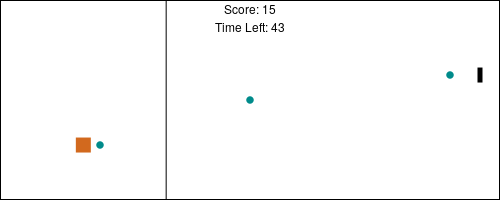
\includegraphics[scale = 0.75]{starcatcher.png}
\end{center}


You should track and report, as the game is running, the number of stars caught and the time left. Display these at the top of the screen. They do not have to be displayed where you see them in the mock up. When the game is over, display a game over screen that reports on the total starts caught and congratulates the player if they caught a majority of the stars thrown.

\section{Versioning}

Just like last time, you need to approach the program in incremental steps, a.k.a. versions. These will focus your energies and determine your grade.

\subsection{Version 0}

Version 0 is a complete ``starter'' for the game. This includes:
\begin{enumerate}
  \item (Lab 10) A complete data definition for the world state along with all necessary auxiliary data definitions.
  \item (Lab 10) Several concrete examples of key game states.
  \item (Lab 10) The signature, purpose, and header for all the top-level event handler functions needed by the game.
\end{enumerate}

\subsection{Version 1}

Complete the design of the following:
\begin{enumerate}
  \item All drawing related functionality including the game over screen
  \item The function(s) that end the game
\end{enumerate}

\subsection{Version 2}

Complete the design of the following:
\begin{enumerate}
  \item The keyboard event handling functions.
  \item Time event handling \textit{without random generation of stars}. This means the thrower moves up and down but does not throw stars.  For testing purposes, just create some already thrown stars by hand.  Stars that are caught and stars that move off the left side of the screen should go away.
\end{enumerate}


\subsection{Version 3}

Complete the design of the following:
\begin{enumerate}
  \item Modify the time handler so that the thrower will randomly throw stars.
\end{enumerate}


\section*{Grading}

Your grade will be determined by two factors: your progress through the versioning determines the letter grade range that is open to you and the quality of your work will determine where you land within that range.

\subsection*{Versions and Grade Ranges}

Successfully completing a version of the program opens up a range of letter grades. Programs that produce syntax errors when run, i.e. they do not actually run, can expect to receive a failing grade. Programs that run but crash often or lack any testing can expect receive something in the D range at best. If you only partially complete a version then you will receive partial credit for that work. Depending on the quality of the work, this might mean as high as a minus grade in the range of the partially completed version.

\begin{tabular}{ll}
\underline{Tier} & \underline{Grade Range} \\
 0 & D \\
 1 & C \\
 2 & B \\
 3 & A
\end{tabular}


\subsection*{Quality}

A high quality program exhibits all the earmarks of intentional, systematic design and good programming style. Program data is appropriately defined. Functions are well documented. Incomplete functions are stubbed as opposed to commented out. Complete functions typically exhibit template structure when applicable. Complete and incomplete functions have a full set of tests. Signatures, purpose statements, tests and function definitions are all appropriately placed.  Function and variable names are helpful and meaningful. Purpose statements are specific and concrete. Indentation of code follows expected Racket standards\sidenote{It's styled like the code in the book.}. Lines are terminated to avoid print wrapping. Comments are used to aid the human reader. Whitespace is used to break up logical blocks of definitions. The degree to which you meet these standards, along with progress within the tier, determines where you fall within the grade range associated with your tier. It is entirely possible the poorly designed and styled code the completes three extensions can get a lower grade than a well designed and styled program that completes one or two extensions. Do not short yourself points by writing sloppy code.


\section*{Important Dates}

\begin{tabular}{ll}
\underline{Date} & \underline{What's Happening} \\
 Monday 4/15 & Work on Version 0 \\
 Tuesday 4/29 & Open Lab Time to For Project Work \\
 Wednesday 5/1 & Due by end of Day
\end{tabular}













\end{document}
